\documentclass[crop, tikz]{standalone}

\usepackage{tikz}
\usepackage{amsmath}
\usepackage{amssymb}
\usepackage[mode=buildnew]{standalone}

\usepackage{xcolor}


\usetikzlibrary{positioning}
\usetikzlibrary{calc}
\usetikzlibrary{fit}
%\usepackage{nicematrix}

\tikzset{set/.style={draw,circle,inner sep=0pt,align=center}}

\definecolor{morange}{RGB}{255,127,14}
\definecolor{mblue}{RGB}{31,119,180}
\definecolor{mred}{RGB}{214,39,40}
\definecolor{mpurple}{RGB}{148,103,189}
\definecolor{mgreen}{RGB}{44,160,44}


\begin{document}
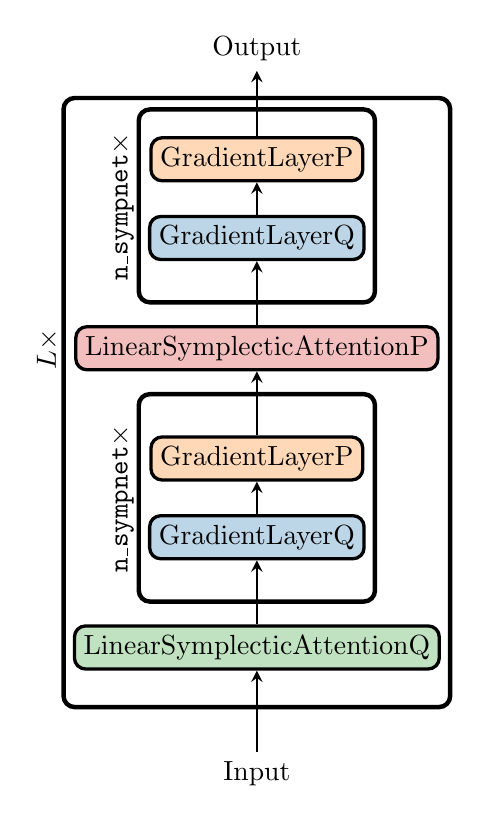
\begin{tikzpicture}[module/.style={draw, very thick, rounded corners, minimum width=15ex},
    gradp/.style={module, fill=morange!30},
    gradq/.style={module, fill=mblue!30},
    attentionq/.style={module, fill=mgreen!30},
    attentionp/.style={module, fill=mred!30},
    arrow/.style={-stealth, thick, rounded corners},
]
\node (input) {Input};
\node[above of=input, attentionq, align=center, yshift=.6cm] (attentionq1) {LinearSymplecticAttentionQ};
\node[above of=attentionq1, gradq, align=center, yshift=.4cm] (gradq1) {GradientLayerQ};
\node[above of=gradq1, gradp, align=center] (gradp1) {GradientLayerP};
\node[above of=gradp1, attentionp, align=center, yshift=.4cm] (attentionp1) {LinearSymplecticAttentionP};
\node[above of=attentionp1, gradq, align=center, yshift=.4cm] (gradq2) {GradientLayerQ};
\node[above of=gradq2, gradp, align=center] (gradp2) {GradientLayerP};
\node[above of=gradp2, yshift=.4cm] (output) {Output};

\draw[arrow] (input) -- (attentionq1);
\draw[arrow] (attentionq1) -- (gradq1); 
\draw[arrow] (gradq1) -- (gradp1);
\draw[arrow] (gradp1) -- (attentionp1); 
\draw[arrow] (attentionp1) -- (gradq2);
\draw[arrow] (gradq2) -- (gradp2); 
\draw[arrow] (gradp2) -- (output);

\coordinate (before_first_sympnet_block) at ($(attentionq1.north)!0.5!(gradq1.south)$);
\coordinate (after_first_sympnet_block) at ($(gradp1.north)!0.5!(attentionp1.south)$);
\coordinate (before_second_sympnet_block) at ($(attentionp1.north)!0.5!(gradq2.south)$);
\coordinate (after_second_sympnet_block) at ($(gradp2.north)!0.2!(output)$);
\coordinate (after_input) at ($(input)!0.6!(attentionq1)$);

\node[fit=(before_first_sympnet_block)(gradq1)(gradp1)(after_first_sympnet_block),draw, ultra thick, rounded corners, label={[rotate=90, yshift=.5em, xshift=3em]left:$\mathtt{n\_sympnet}\times$}] (sympnet1) {};
\node[fit=(before_second_sympnet_block)(gradq2)(gradp2)(after_second_sympnet_block),draw, ultra thick, rounded corners, label={[rotate=90, yshift=.5em, xshift=3em]left:$\mathtt{n\_sympnet}\times$}] (sympnet2) {};
\node[fit=(after_input)(attentionq1)(attentionp1)(sympnet1)(sympnet2), draw, ultra thick, rounded corners, label={[rotate=90, yshift=.5em, xshift=3em]left:$L\times$}] (block) {};
\end{tikzpicture}
\end{document}